\chapter{Umsetzung und Implementation}
\label{chap:implementation}


%%%%%%%%%%%%%%%%%%%%%%%%%%%%%%%%%%%%%%%%%%%%%%%%%%%%%%%%%%%%
\section{Initialisierung und Beacon-Daten}
\label{sec:implementation:initandbeacon}
%%%%%%%%%%%%%%%%%%%%%%%%%%%%%%%%%%%%%%%%%%%%%%%%%%%%%%%%%%%%
Die Funktionen zum Positionsupdate und zur Erkennung der Beacons werden dabei im \emph{LocationManager} verwaltet.
In der \emph{LocationManagerDelegate} lassen sich dabei die Aktionen bestimmen, welche bei verschiedenen Events ausgeführt werden.

In Listing \ref{lst:locationmanager_objc} wird die Initialisierung eines LocationManager gezeigt, welcher eine Genauigkeit von einem Kilometer haben soll und bei Positionsänderungen von mehr als 500 Metern aktualisiert wird.

  \begin{listing}[htb!]
    \insertminted{objc}{code_examples/locationManager.m}
    \caption{Beispielinitialisierung für einen LocationManager.}
    \label{lst:locationmanager_objc}
  \end{listing}

%%%%%%%%%%%%%%%%%%%%%%%%%%%%%%%%%%%%%%%%%%%%%%%%%%%%%%%%%%%%
\section{Ansatz zur Positionsbestimmung}
\label{sec:implementation:positioning}
%%%%%%%%%%%%%%%%%%%%%%%%%%%%%%%%%%%%%%%%%%%%%%%%%%%%%%%%%%%% 
Bei der Positionsbestimmung geht es um die Bestimmung des aktuellen Ortes in Echtzeit und das auf bis zu 10cm genau. Bei der Positionsangabe handelt es sich hier um eine zweidimensionale Position, da dies für unsere Zwecke ausreicht.

Bei der Positionsbestimmung wurden zwei verschiedene Ansätze untersucht. Zum einen die Trilateration, welche eine Positionierung mittels Entfernungen zu verschiedenen Fixpunkten ermöglicht und zum Anderen die Positionierung mittels Fingerprinting, welches eine Datenbank mit sogenannten Fingerprints, also vorher aufgezeichneten Messwerten und damit verbundenen Positionsdaten, voraussetzt und darüber die aktuelle Position bestimmt.

Die Positionsbestimmung soll dabei in einem 2D-Raum erfolgen, da die Höhe vernachlässigt werden kann. In der realen Welt kann die Höhe ebenfalls vernachlässigt werden, da dort Stockwerke meist einen deutlichen Höhenunterschied aufweisen, sodass dieser über andere Faktoren eindeutig bestimmt werden kann.


%%%%%%%%%%%%%%%%%%%%%%%%%%%%%%%%%%%%%%%%%%%%%%%%%%%%%%%%%%%%
\section{Trilateration}
\label{sec:implementation:trilateration}
%%%%%%%%%%%%%%%%%%%%%%%%%%%%%%%%%%%%%%%%%%%%%%%%%%%%%%%%%%%%
Die Trilateration ist eine Methode zur Bestimmung der aktuellen Position. Im Gegensatz zur Triangulation, welche die Position anhand der Winkelgrößen zwischen verschiedenen Fixpunkten bestimmt, wird bei der Trilateration die Position durch die Abstände zu den Fixpunkten bestimmt. 

Bei der Trilateration wird der Abstand zu einem Fixpunkt genutzt, um die Position des Objektes zu bestimmen. Das Objekt muss dabei auf einer Kreisbahn um den Fixpunkt liegen, welche den Radius des zuvor bestimmten Abstand besitzt. Um nun einen genauen Standpunkt zu bestimmen, sind mindestens drei Fixpunkte und die dazugehörige Abstände nötig, da so im zweidimensionalem Raum ein eindeutiger Schnittpunkt entsteht.

\begin{figure}[htb!]
	\centering
	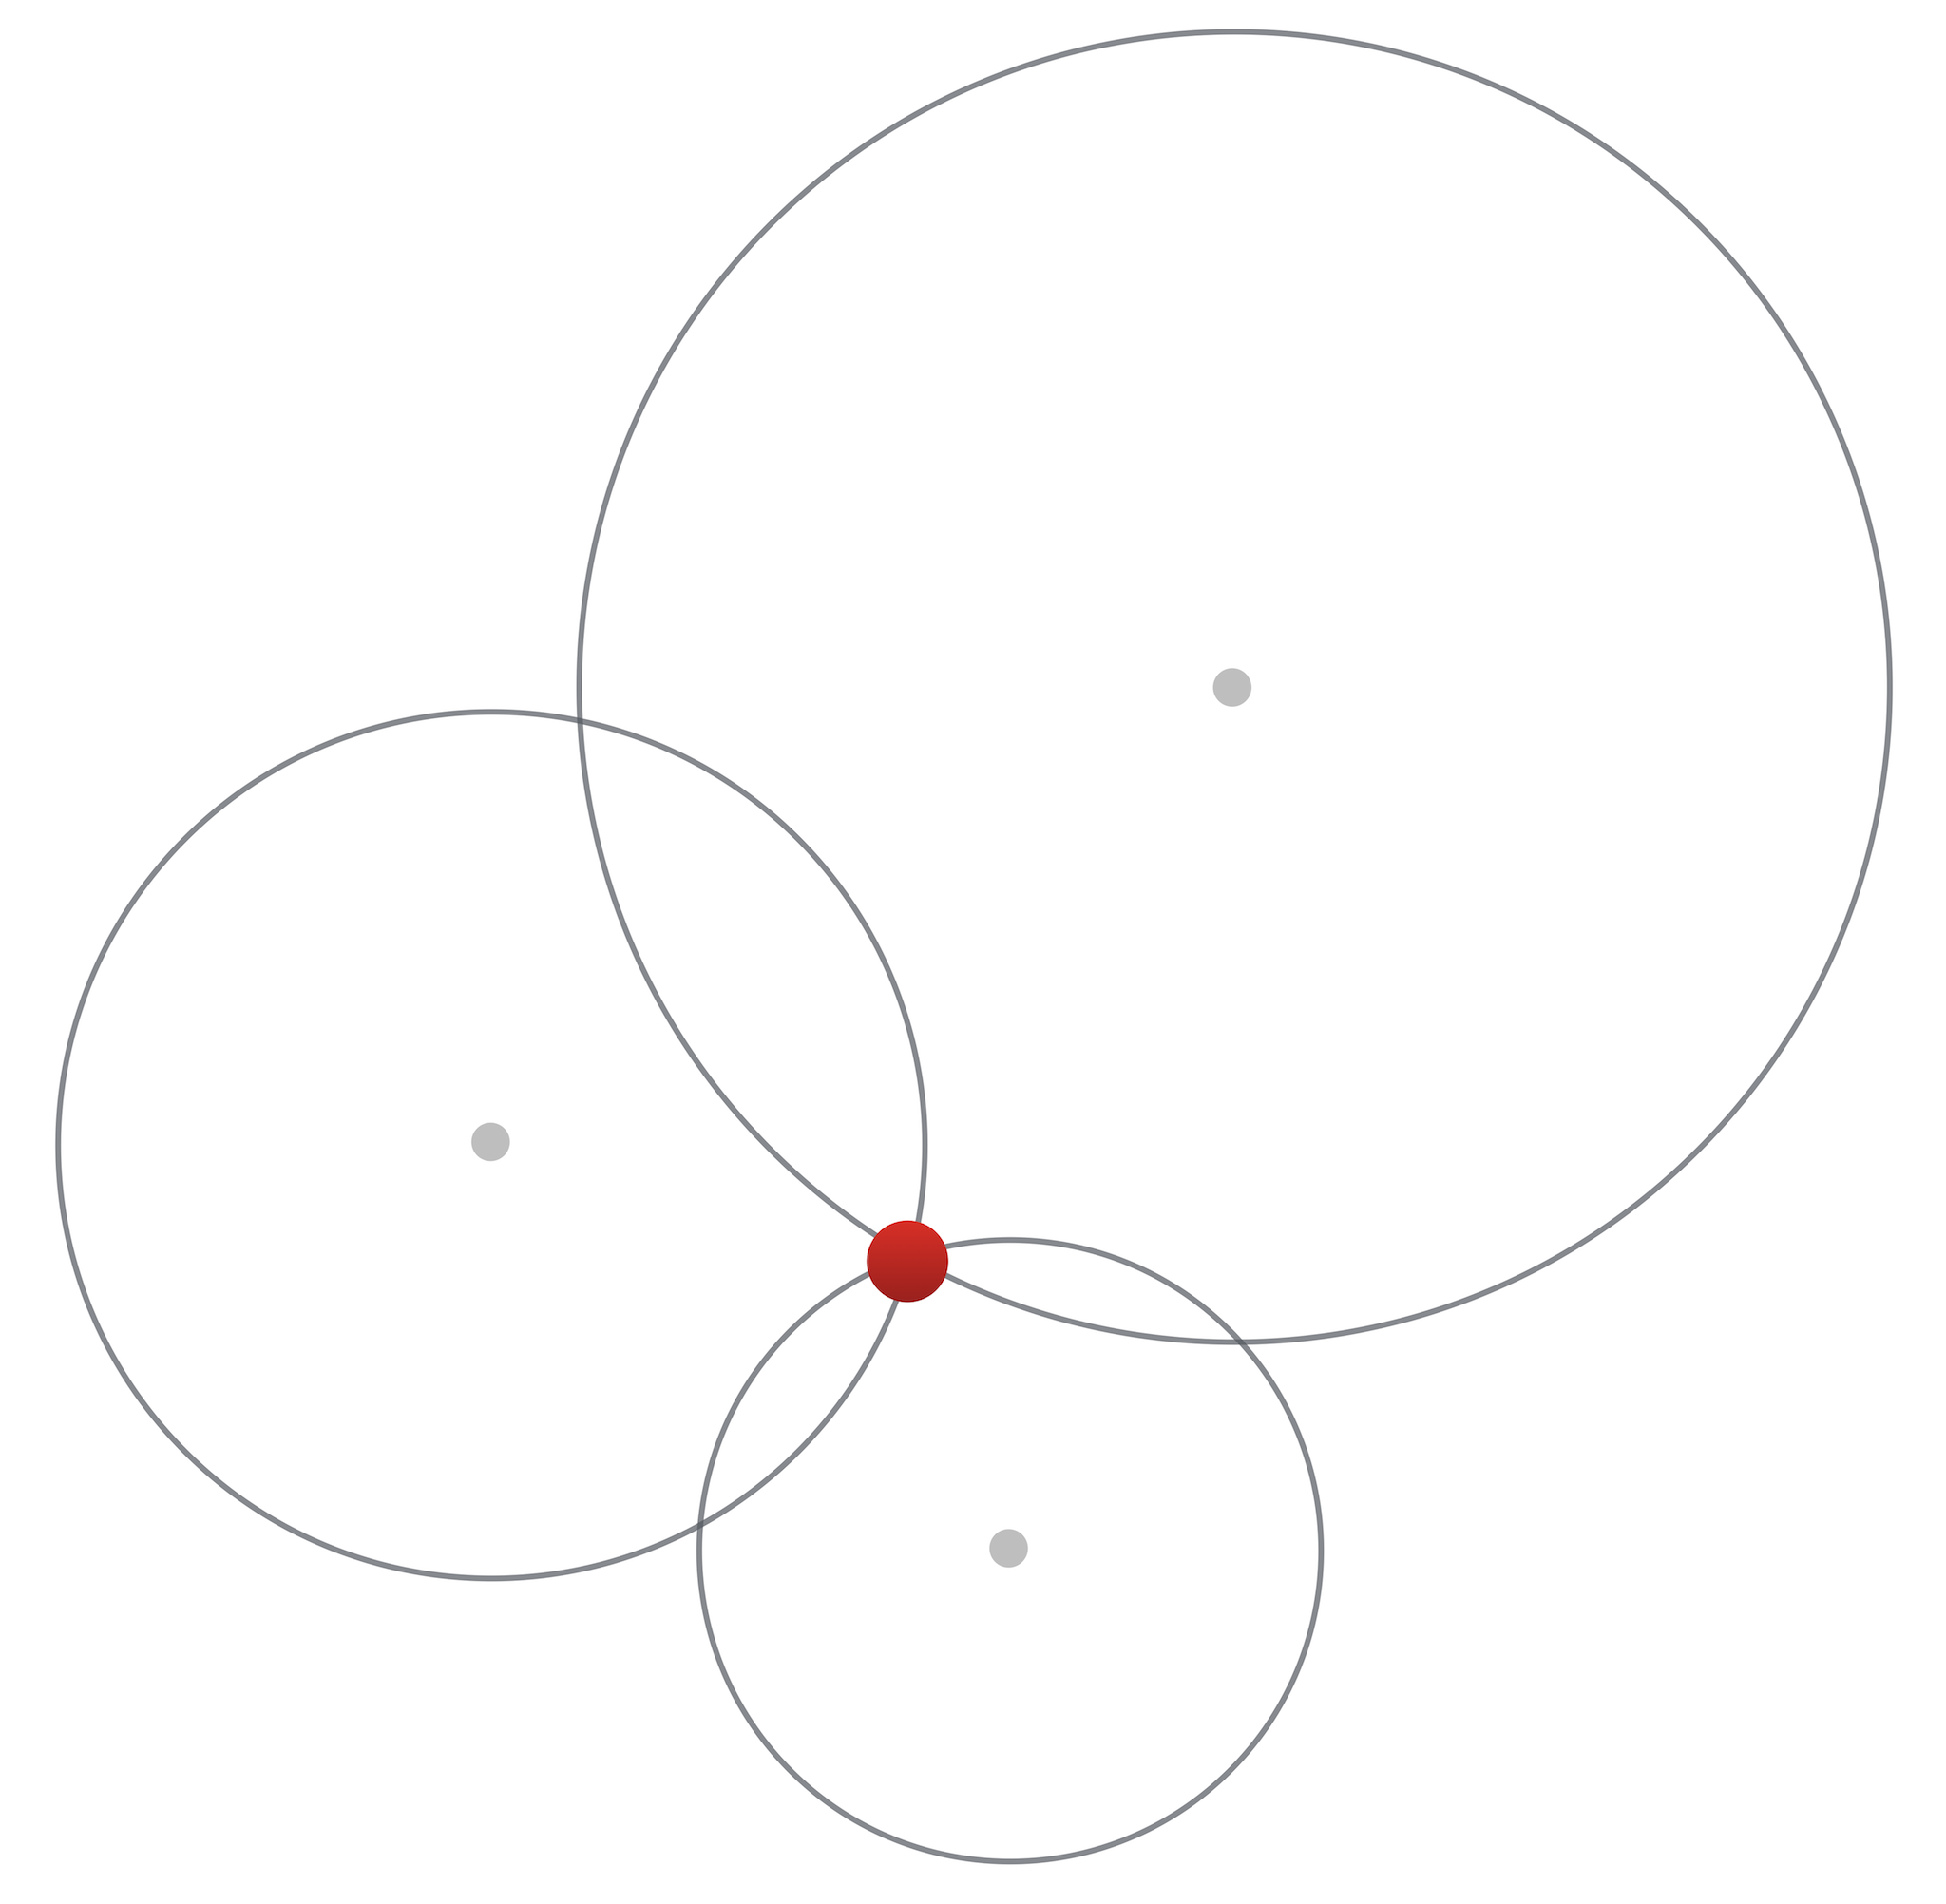
\includegraphics[scale=1.5]{trilateration}
	\caption{Funktionsprinzip der Trilateration}
	\label{trilateration-accurate}
\end{figure}

In Abbildung \ref{trilatertion-accurate} sieht man dabei die Funktionsweise der Trilateration bei genauer Abstandsbestimmung. In realen Messungen und Positionsbestimmungen ist es jedoch nicht möglich genaue Abstände zu bestimmen, da es immer zu Messungenauigkeiten kommen kann.
Bei solchen ungenauen Messungen ist es nun nicht mehr möglich einen genauen Schnittpunkt zu finden. 

Um diese Ungenauigkeit auszugleichen wird das Verfahren entsprechend angepasst. Dabei werden Geraden durch die Schnittpunkte der einzelnen Umkreise gelegt. Dadurch entsteht zwischen den Geraden ein neuer Schnittpunkt, welcher die aktuelle Position repräsentiert. Dieses Verfahren wird in Abbildung \ref{trilateration-inaccurate} dargestellt.

\begin{figure}[htb!]
		\centering
	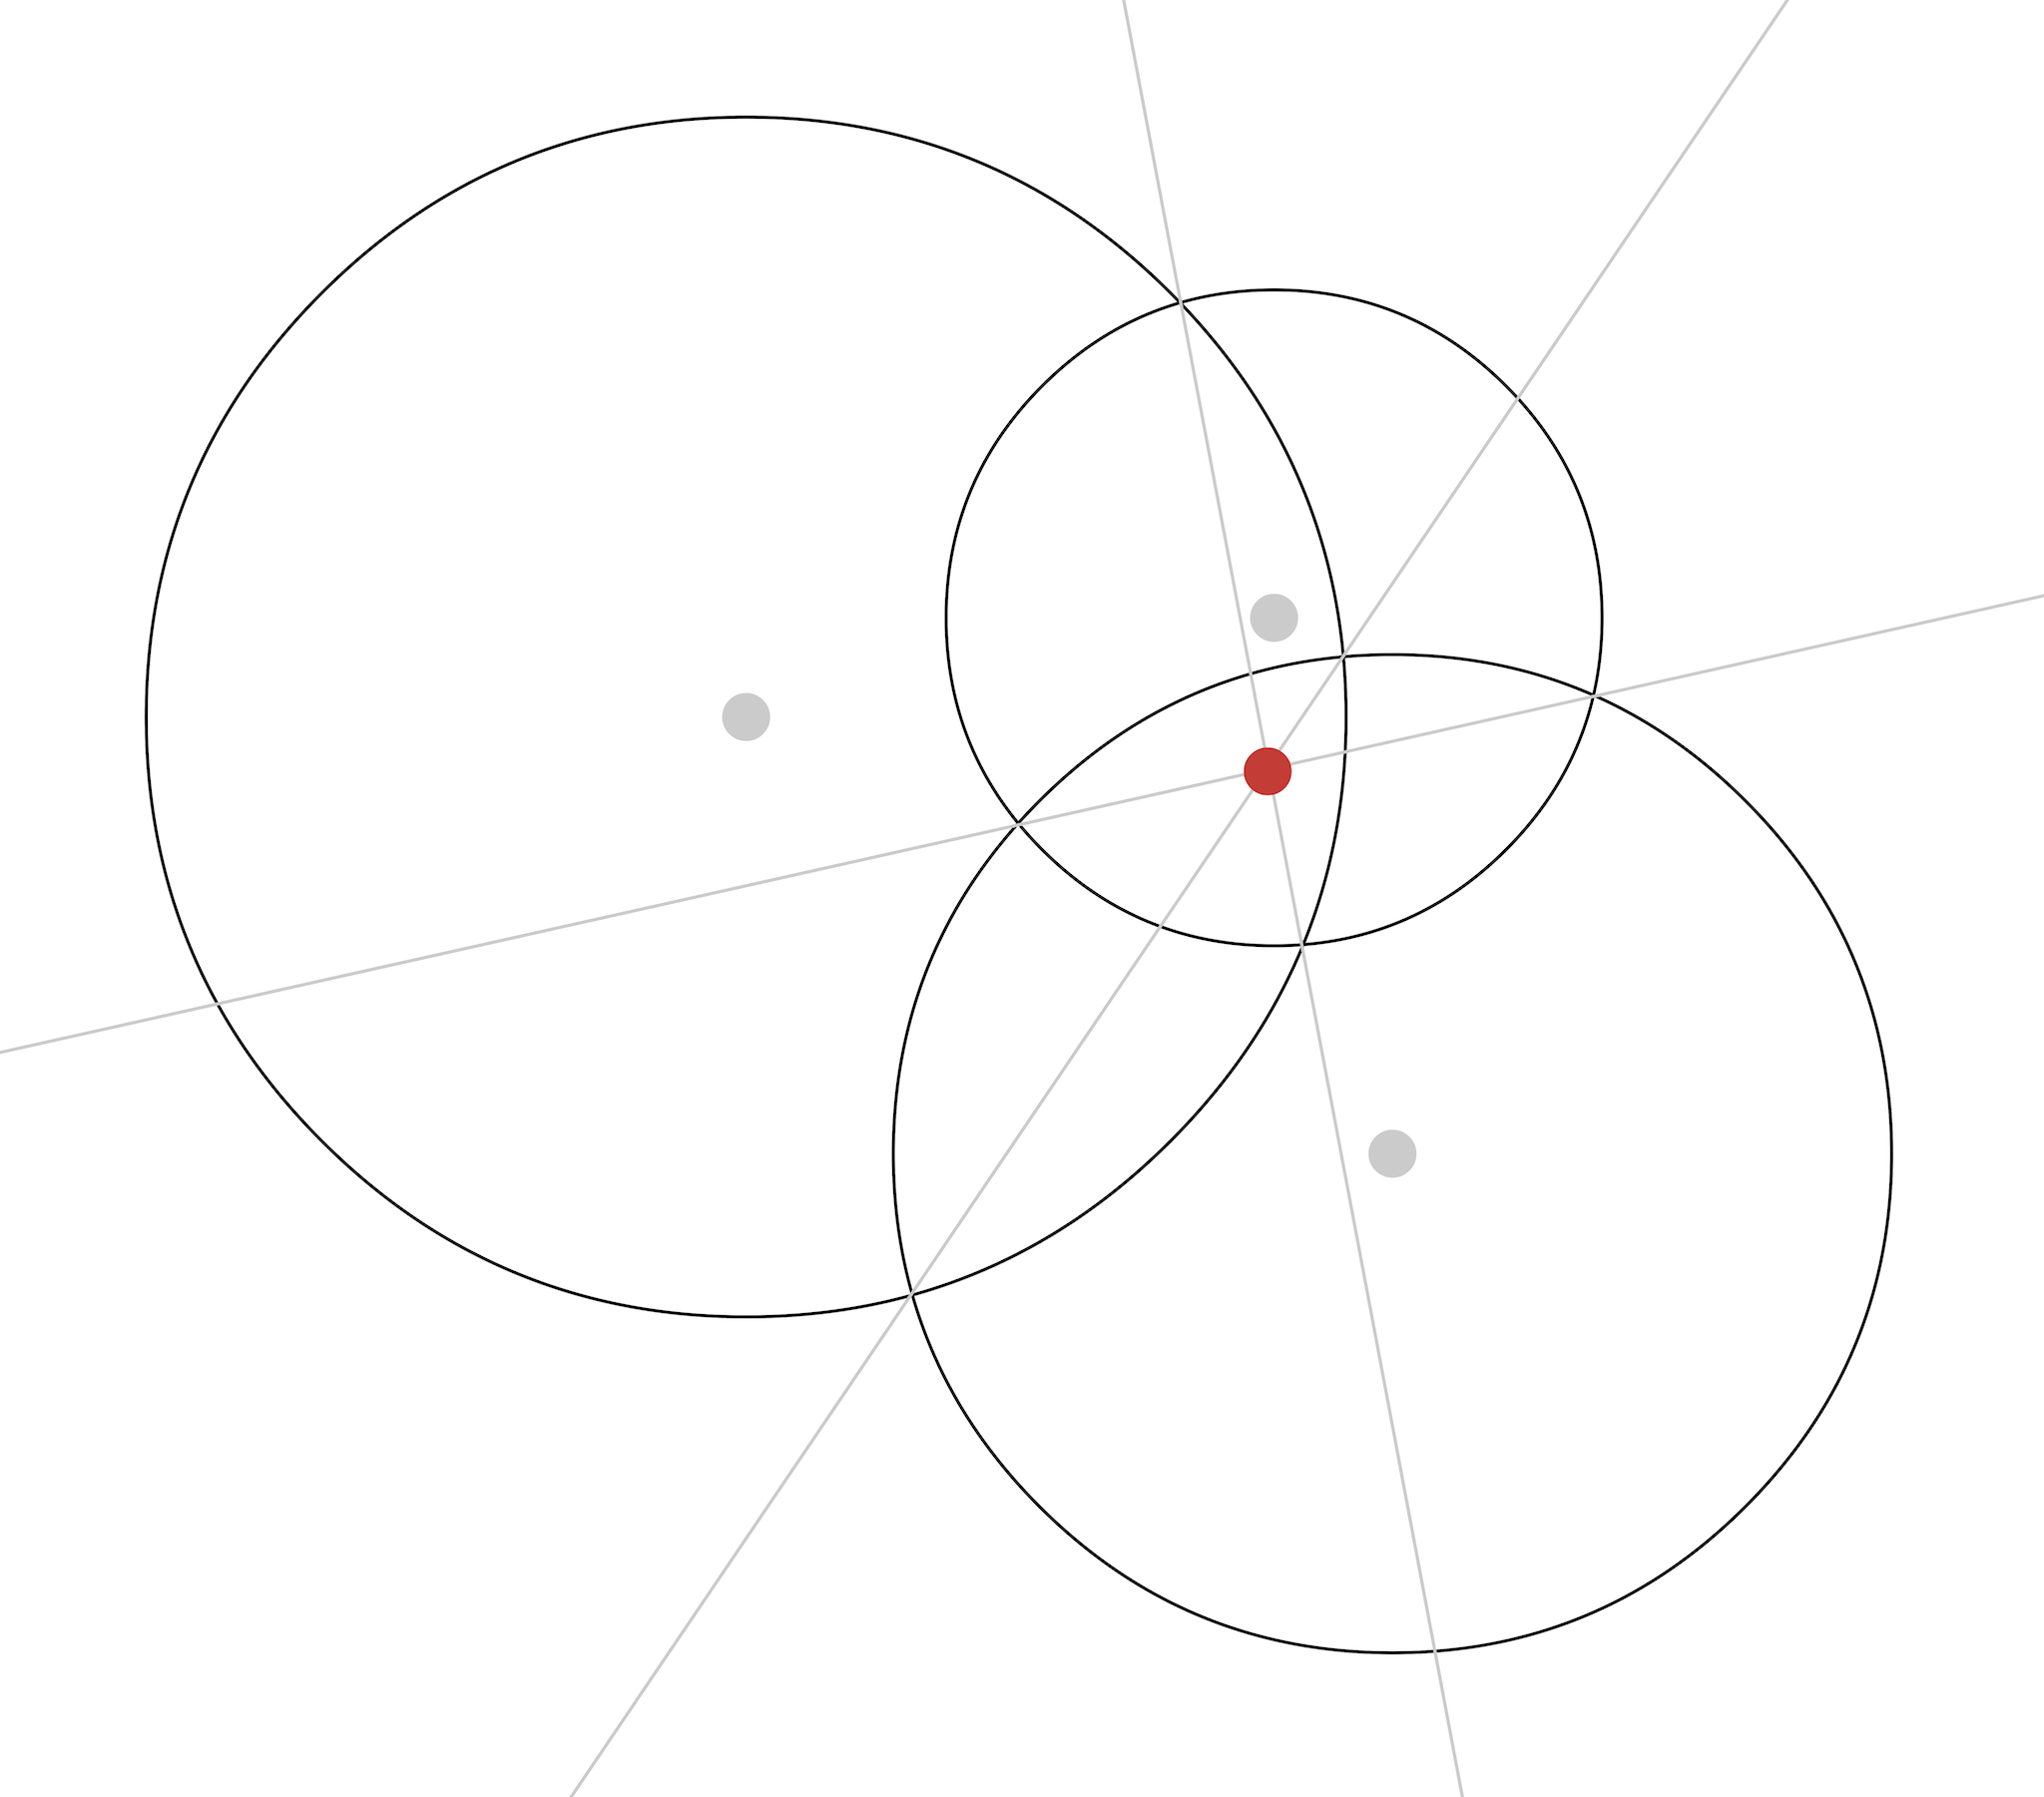
\includegraphics[scale=1.5]{trilateration-inaccurate}
	\caption{Trilateration bei ungenauen Abständen zu den Fixpunkten}
	\label{trilateration-inaccurate}
\end{figure}

Damit ist es möglich auftretende Ungenauigkeiten zu kompensieren und trotzdem eine genaue Positionsbestimmung durchzuführen.

Bei der genutzten iBeacons beziehungsweise Bluetooth-Technologie ist eine genaue Entfernungsangabe jedoch nicht vorgesehen, wodurch das Verfahren der Trilateration nicht direkt angewandt werden kann. Dafür muss zunächst ein Ersatzindikator für die Entfernungsmessung bestimmt werden.
Bei der Bluetooth-Technologie bietet sich dafür die Signalstärke an.
Dabei wird die Tatsache genutzt, dass die Signalstärke mit zunehmendem Abstand sinkt und man somit aus der aktuellen Signalstärke auch die aktuelle Entfernung bestimmen kann. 
Das Verhältnis zwischen Entfernung und Signalstärke bei elektromagnetischen Wellen wird durch das Abstandsgesetz beschrieben, welches besagt, das die Signalstärke quadratisch zum Abstand abnimmt.

\begin{equation}
	\text{\emph{Signalstärke}} = \text{\emph{Ausgangssignalstärke}}/\text{\emph{Entfernung}}^2
\end{equation}

Diese Annahme mag bei freien Flächen korrekt sein, in Innenräumen kommen jedoch weitere Faktoren hinzu. 
Durch Wände und Hindernisse im Raum, wie zum Beispiel Schränke, Regale, usw., kommt es dort zu einer Dämpfung des Signals, wodurch die Signalstärke beeinflusst wird. Des Weiteren kann es in Innenräumen auch zu Streuung und Reflexionen kommen, welche das Signal zusätzlich verfälschen.

Diese Annahme bestätigt sich auch bei den Messungen. Diese zeigen, dass die gemessene Signalstärke nicht, wie angenommen, mit der Entfernung stetig abnimmt, sondern sehr stark schwankt, wodurch keine genaue Entfernungsbestimmung durchgeführt werden kann.

Die Methode der Trilateration wurde auf Grund der fehlenden Genauigkeit verworfen. 

%%%%%%%%%%%%%%%%%%%%%%%%%%%%%%%%%%%%%%%%%%%%%%%%%%%%%%%%%%%%
\section{Fingerprinting}
\label{sec:implementation:fingerprinting}
%%%%%%%%%%%%%%%%%%%%%%%%%%%%%%%%%%%%%%%%%%%%%%%%%%%%%%%%%%%%
Das Fingerprinting ist ein Verfahren der Positionsbestimmung auf der Grundlage von zuvor erhobenen Messwerten, den sogenannten Fingerprints.
Die Funktionsweise des Fingerprintings unterscheidet sich grundlegend von der Methode der Trilateration, da hierbei keine direkte Berechnung der Position über Entfernungsgrößen geschieht, sondern die Positionierung über, in einer Datenbank abgelegten Erfahrungswerten geschieht.

Um dieses Verfahren umzusetzen muss der Messraum, in welchem die Positionierung statt finden soll, zunächst in ein Gitternetz eingeteilt werden, wobei jede Zelle des Gitters eine mögliche Position im Raum repräsentiert. Die Größe dieser Zellen ist prinzipiell frei wählbar, wird jedoch im wesentlichen durch zwei Faktoren bestimmt. 
Zum einen die gewünschte Genauigkeit. Da jede Zelle eine mögliche Position repräsentiert, wird durch die Größe der Zellen auch die Genauigkeit der Position bestimmt. Daraus ergibt sich das die Genauigkeit zunimmt, wenn die Zellengröße verkleinert wird.
Der zweite Faktor bei der Wahl der Zellengröße, ist die eindeutige Bestimmung der Zelle. Dies ist darauf zurückzuführen, dass bei kleineren Zellen die Differenzen zwischen den einzelnen Zellen ebenfalls abnehmen. Um nun eine genaue Bestimmung der Zelle zu ermöglichen, sollte jede Zelle so groß gewählt werden, dass dies noch möglich ist.

Daher sollte die Zellengröße so gewählt werden, dass eine gute Unterscheidbarkeit zwischen den einzelnen Zellen gewährleistet ist, hinzu jedoch eine möglichst genaue Positionsbestimmung erzielt werden kann.


Das Fingerprinting besteht im Wesentlichen aus zwei Phase.

Die erste Phase ist die sogenannte \emph{Trainingsphase}. Dabei werden die sogenannten \emph{Fingerprints} gesammelt, welche letztlich zur Positionsbestimmung genutzt werden. 
In der Trainingsphase werden daher, für jede Zelle unseres Messraumes eine Reihe von Fingerprints gesammelt. Die Anzahl der Fingerprints sollte dabei relativ groß sein, sodass Messfehler kompensiert werden können. 
Ein Fingerprint kann sich dabei aus verschiedenen Daten zusammensetzen. 
In diesem Fall besteht ein Fingerprint aus der aktuellen Zellennummer beziehungsweise der Zellenkoordinate, einem Zeitstempel mit aktuellem Datum und der Uhrzeit und den Signalstärken zu den verschiedenen, in Reichweite befindlichen Sendestationen, welches in diesem Fall die iBeacons sind.

Die Sammlung der Fingerprints muss für jede Zelle geschehen und macht die Trainingsphase daher sehr zeitaufwendig. 

Die der zweiten Phase, auch \emph{Onlinephase} genannt, werden die zuvor gesammelten Informationen verwendet um die aktuelle Position zu bestimmen. 
Dafür werden die gesammelten Fingerprints mit den aktuell gemessenen Signalstärken verglichen. Wenn eine Übereinstimmung gefunden wird, wird die Position des passenden Fingerprints als aktuelle Position angenommen.

\todo{Einfügen von Zeichnung welche Zellen und Fingerprints verdeutlicht}

%%%%%%%%%%%%%%%%%%%%%%%%%%%%%%%%%%%%%%%%%%%%%%%%%%%%%%%%%%%%
\subsection{Positionsbestimmung}
\label{sec:implementation:fingerprinting:positioning}
%%%%%%%%%%%%%%%%%%%%%%%%%%%%%%%%%%%%%%%%%%%%%%%%%%%%%%%%%%%%
Bei der Positionsbestimmung mittels Fingerprinting gibt es verschiedene Ansätze.
Das erste Verfahren vergleicht alle Fingerprints in der Datenbank mit den aktuellen Messwerten und bestimmt damit die aktuelle Position.
Eine weitere Möglichkeit besteht darin, den Durchschnittswert der Fingerprints zu bilden um diesen dann mit den aktuellen Werten zu vergleichen.
Die letzte untersuchte Möglichkeit ist die der Wahrscheinlichkeitsverteilung der Werte. Hier wird über die Wahrscheinlichkeitswerte der einzelnen Messwerte die aktuelle Position bestimmt.

%%%%%%%%%%%%%%%%%%%%%%%%%%%%%%%%%%%%%%%%%%%%%%%%%%%%%%%%%%%%
\subsection{Einfache Positionsbestimmung mittels Nearest-Neighbor-Verfahren}
\label{sec:implementation:fingerprinting:positioning:naiv}
%%%%%%%%%%%%%%%%%%%%%%%%%%%%%%%%%%%%%%%%%%%%%%%%%%%%%%%%%%%%
Bei der einfachen und naiven Bestimmung der aktuellen Position, werden alle zuvor gesammelten Fingerprints mit den aktuell gemessenen Signalstärken verglichen. Dies führt dazu, dass bei größeren Fingerprint-Datenbanken auch die Rechenzeit und der Energieverbrauch steigt. 

Bei dem Vergleich der Messwerte mit den gespeicherten Fingerprints wird das Nearest-Neighbor-Verfahren verwendet. Dabei werden sowohl die aktuellen Messwerte, als auch die Fingerprints als Vektoren aus den Signalstärken zusammengefasst und aus diesen Vektoren wird die jeweilige Entfernung der beiden Werte berechnet. Die einzelnen Signalstärken-Werte sind die Werte von allen in Reichweite befindlichen Beacons.

Bei der Berechnung wird dabei für jeden Fingerprint ein Vektor erzeugt, welcher die Signalstärken zu den in Reichweite befindlichen Beacons beinhaltet.
Die Signalstärke für die Beacons wird hier als \emph{FSig} bezeichnet, wobei ein Zusatz angibt auf welches Beacon sich der Wert bezieht, zum Beispiel \emph{FSigB1} für die Signalstärke des Beacons 1.
Die Signalstärke der aktuellen Messung wird mit \emph{MSig} abgekürzt und ebenfalls um den Identifikator des Beacons erweitert.


\begin{equation}
	\begin{pmatrix}
		FSigB1 \\
		FSigB2 \\
		FSigB3 \\
		...
	\end{pmatrix} -
	\begin{pmatrix}
		MSigB1 \\
		MSigB2 \\
		MSigB3 \\
		...
	\end{pmatrix}
	= 
	\begin{pmatrix}
		FSigB1 - MSigB1 \\
		FSigB2 - MSigB2 \\
		FSigB3 - MSigB3 \\
		...
	\end{pmatrix}
\end{equation}

\begin{equation}
	\begin{pmatrix}
		FSigB1 - MSigB1 \\
		FSigB2 - MSigB2 \\
		FSigB3 - MSigB3 \\
		...
	\end{pmatrix}
	=
	\begin{pmatrix}
		Diff1 \\
		Diff2 \\
		Diff3 \\
		...
	\end{pmatrix}
	\widehat{=}
	\sqrt{Diff1^2 + Diff2^2 + Diff3^2 + ...}
\end{equation}

Aus den Differenzen beziehungsweise die Abstände zwischen den einzelnen Signalstärke-Vektoren lässt sich nun der Nearest-Neighbor bestimmen und damit die wahrscheinliche Position im Raum.

%%%%%%%%%%%%%%%%%%%%%%%%%%%%%%%%%%%%%%%%%%%%%%%%%%%%%%%%%%%%
\subsubsection{Probleme}
\label{sec:implementation:fingerprinting:positioning:naiv:problems}
%%%%%%%%%%%%%%%%%%%%%%%%%%%%%%%%%%%%%%%%%%%%%%%%%%%%%%%%%%%%
Bei dem Standard Nearest-Neighbor-Verfahren kommt es jedoch zu einigen Problemen. 
Die Masse der zu überprüfenden Daten kann, je nach der Größe der Fingerprint-Datenbank, sehr groß werden. Bei sehr großen Datenmengen kann es zu einer längeren Laufzeit bei der Überprüfung der Fingerprints kommen und ausserdem wird mehr Systemspeicher belegt. 
Eine Möglichkeit dies zu beheben, wäre die Verlagerung der Berechnungen auf einen Server, welche als Ergebnis die aktuelle Position liefert. Die zu übertragenden Daten dabei sind sehr gering, da es sich nur um die aktuellen Beacon-Signalstärken handelt beziehungsweise die aktuelle Position, welche vom Server zurückgesendet wird. 
Ausserdem würde die Rechenlast komplett von iPhone genommen, was sich positiv auf die Batterielaufzeit und Performance auswirkt.

Ein weiteres Problem sind Messfehler beziehungsweise Messausreißer, welche das Ergebnis verfälschen können. So werden auch Ausreißer in das Nearest-Neighbor-Verfahren mit einbezogen, wodurch die Berechnung der aktuellen Position verfälscht werden kann.

In der Realität ist das Standard-Nearest-Neighbor-Verfahren nicht problemlos möglich, da die Positionsangabe stark schwankt und zwischen einzelnen Positionen springt.

Daher wurde überlegt, wie dieses Problem behoben werden könnte. Dies wurde so gelöst, dass statt aller Fingerprint-Wert nur der durchschnittliche Wert der Signalstärke eines Beacons genutzt wird.


%%%%%%%%%%%%%%%%%%%%%%%%%%%%%%%%%%%%%%%%%%%%%%%%%%%%%%%%%%%%
\subsection{Nearest-Neighbor-Verfahren mit Mittelwerten}
\label{sec:implementation:fingerprinting:positioning:avg}
%%%%%%%%%%%%%%%%%%%%%%%%%%%%%%%%%%%%%%%%%%%%%%%%%%%%%%%%%%%%
Der zweite Ansatz arbeitet ähnlich wie das zuvor erklärte Verfahren, nutzt jedoch nicht die komplette Datenbank der Fingerprints. 
Stattdessen wird für jede Zelle ein Mittelwert über alle Fingerprints der vorhandenen Beacons berechnet und dieser für die Bestimmung der Position verwendet.
Dieser Mittelwert muss dabei nur bei einer Änderung der grundlegenden Fingerprint-Datenbank angepasst werden, wodurch der Rechenaufwand niedriger gehalten wird, da bei jeder Positionsbestimmung nur auf den Mittelwert zugegriffen werden muss.
Ausserdem wird der Einfluss von Störungen und Messungenauigkeiten der Fingerprints verringert.

Bei der Implementierung wurden zwei Mittelwerte getestet. Zum einen der Median, welcher den mittleren Wert einer sortierten Reihe aller Werte nutzt und zum anderen das arithmetische Mittel, welcher alles Werte aufaddiert und dann durch die Anzahl der Werte dividiert.

\begin{equation}
	RSSI_{avg} = \frac{RSSI_{1} + RSSI_{2} + ... + RSSI_{n}}{n}
\end{equation}

Der arithmetische Mittelwert lässt sich sehr leicht berechnen und schafft es kleinere Messungenauigkeiten zu beseitigen. Falls jedoch sehr starke Messfehler einfließen, können diese das arithmetische Mittel deutlich verfälschen.

Im Gegensatz dazu ist der Median deutlich robuster als das arithmetische Mittel.

Der Median errechnet sich dabei wie folgt: 

\begin{equation}
	\begin{split}
	\text{\emph{Für }}RSSI \text{\emph{ gilt: }} RSSI_{1} \leq RSSI_{2} \leq ... \leq RSSI_{n} \\
	RSSI_{median}=\begin{cases}
	RSSI_{\frac{n+1}{2}} & \text{für } n \text{ ungerade}\\ \\
	\frac{RSSI_{\frac{n}{2}} + RSSI_{\frac{n}{2}+1}}{2} & \text{für } n \text{ gerade} \\
	\end{cases}
	\end{split}
\end{equation}

Bei der Berechnung wird klar, warum Messfehler keinerlei Auswirkungen haben. Da beim Median, der mittlere Wert der sortierten Reihe genutzt wird, spielen Messfehler, welche sich am Anfang oder Ende der Reihe befinden, keine Rolle.

Im Testeinsatz war der Unterschied zwischen Median und arithmetischem Mittel jedoch zu vernachlässigen. 


%%%%%%%%%%%%%%%%%%%%%%%%%%%%%%%%%%%%%%%%%%%%%%%%%%%%%%%%%%%%
\subsection{Prohabilistisches Verfahren}
\label{sec:implementation:fingerprinting:positioning:probability}
%%%%%%%%%%%%%%%%%%%%%%%%%%%%%%%%%%%%%%%%%%%%%%%%%%%%%%%%%%%%
Der letzte untersuchte Ansatz war ein prohabilistisches Verfahren, welches die Wahrscheinlichkeiten einer bestimmten Signalstärke eines Beacons als Referenz-Wert für die Positionbestimmung nutzt. Dabei wurde für die Berechnung der Wahrscheinlichkeiten und Bestimmung der aktuellen Position das Verfahren von \citet{wifiFingerprintProbability} verwendet, welche das Fingerprinting mit Hilfe von Wireless LAN-Routern verwenden.

Da das Fingerprinting mit Wireless LAN auch auf den Signalstärken der Wireless LAN-Basisstationen basiert, lässt sich das Verfahren auch auf andere Technologien, welche die Signalstärke zur Positionsbestimmung nutzen, übertragen.

Während der initialen Offline-Phase wird, nachdem die Fingerprints gesammelt wurden, eine Wahrscheinlichkeitsverteilung der Signalstärken für jedes Beacon in jeder Zelle erstellt. Diese wird später als Vergleichswert genutzt, um die Ähnlichkeit der Signalstärken zu bestimmen.

\begin{figure}[htb!]
		\centering
	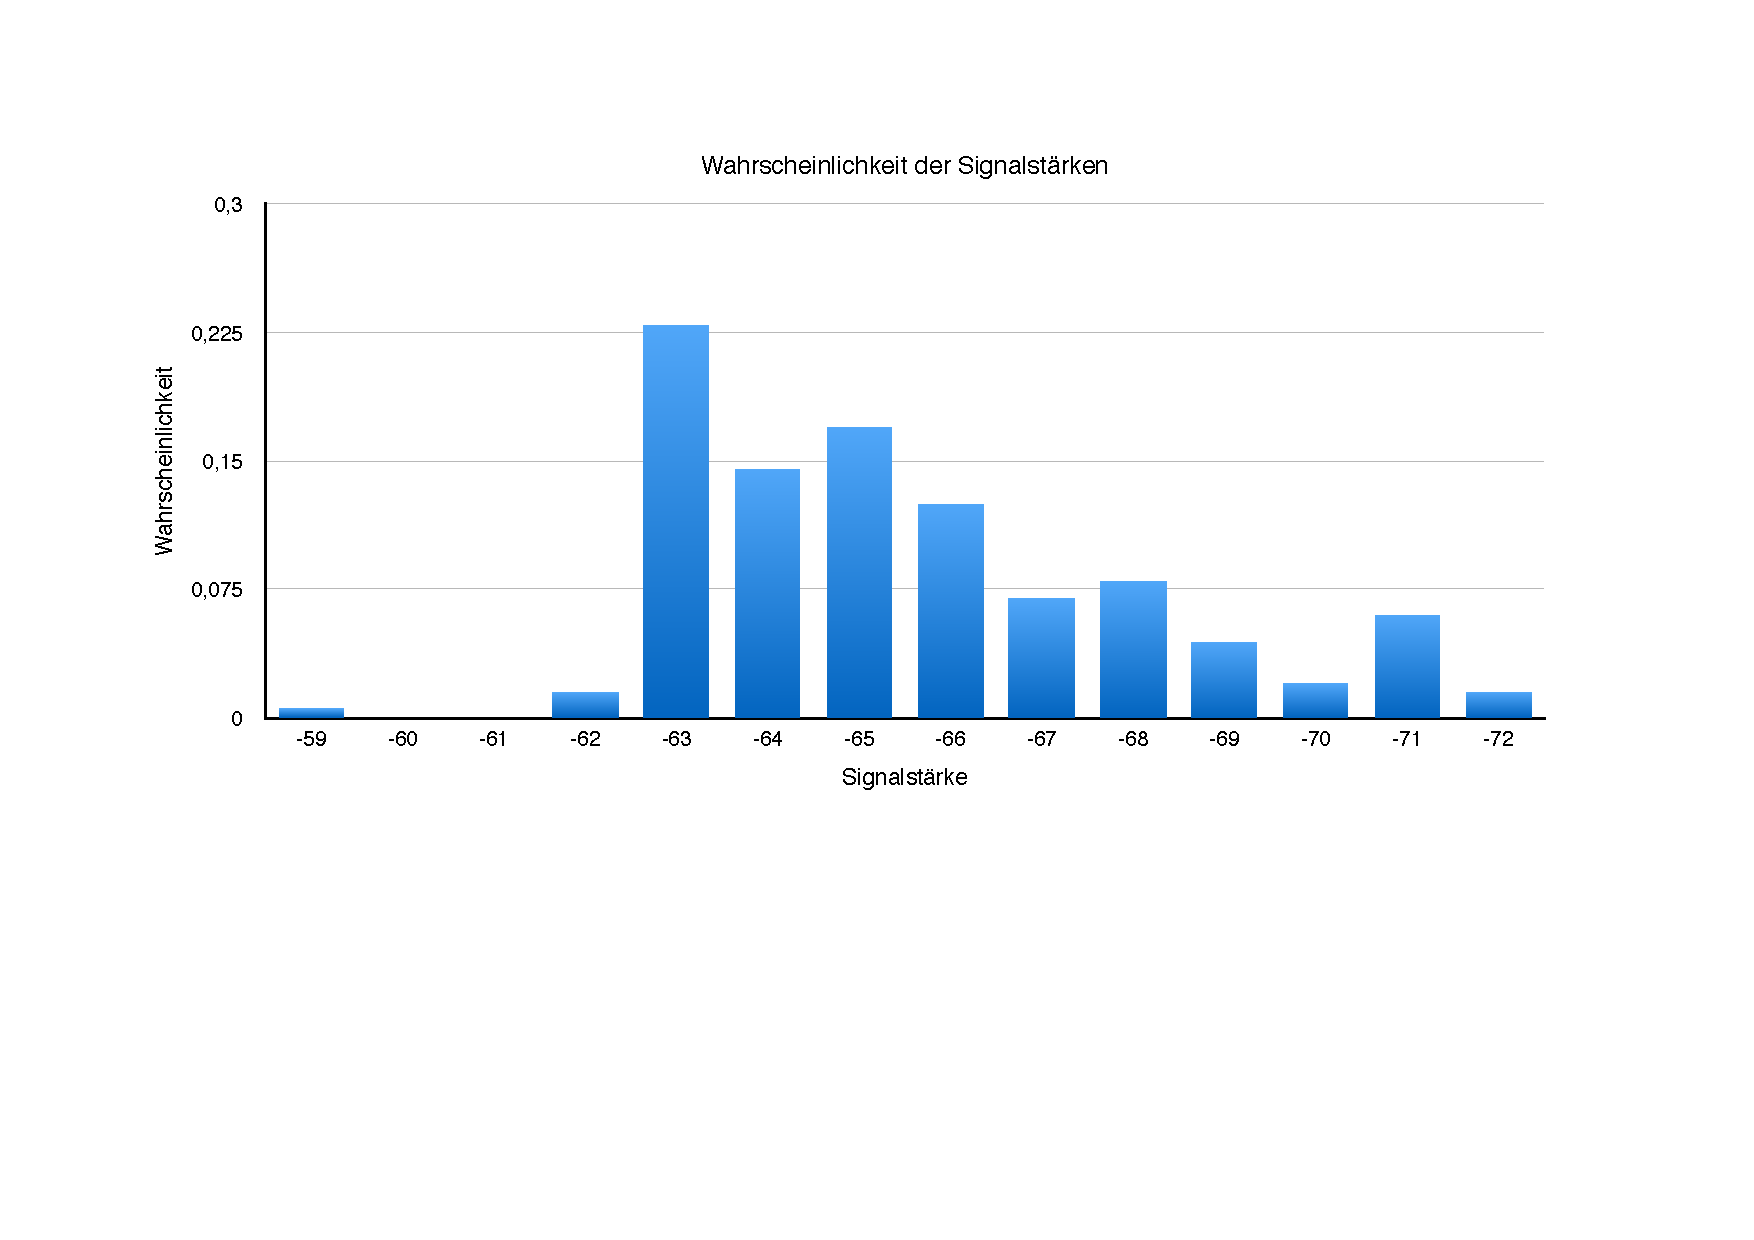
\includegraphics[scale=0.2]{probability_signal_strength}
	\caption{Wahrscheinlichkeitsverteilung von Signalstärke bei einem Beacon}
	\label{probability-signal-strength-beacon}
\end{figure}

Danach folgt die Online-Phase in der die aktuelle Position bestimmt werden soll. Dafür werden die aktuellen Signalstärken der Beacons gemessen und gespeichert, um von diesen Werten ebenfalls eine Wahrscheinlichkeitsverteilung zu berechnen. Die Anzahl der Werte, welche in die Wahrscheinlichkeitsverteilung einfließen ist dabei sehr wichtig.
Für eine statische Positionsbestimmung sollte die Anzahl der letzten gespeicherten Werte groß gewählt werden, da es hier keine Echtzeit-Änderung der Position geschieht.
Für unsere Anwendung der Echtzeit-Positionsbestimmung ist ein relativ schnelles aktualisieren der Position jedoch essenziell. Daher muss hier ein Kompromiss aus akkurater Positionsbestimmung und Echtzeit-Fähigkeit gefunden werden.

Die Wahrscheinlichkeitsverteilung der aktuell gemessenen Werte muss nun mit den Verteilungen aller Zellen verglichen werden und deren Ähnlichkeit muss bestimmt werden. Dafür wird die Bhattacharyya-Distanz genutzt, welche die Ähnlichkeit zweier Wahrscheinlichkeitsverteilungen beschreibt. 
Diese Distanz muss für jede Zelle errechnet werden. 
Dafür muss zunächst der Bhattacharyya-Koeffizient $B_{b, c}$ für jedes Beacon $b$ einer Zelle $c$ berechnet werden.

\begin{equation}
	B_{b, c} = \sum_{s \in [s_{min},s_{max}]} \sqrt{P_{b}^{c}(s) \cdot Q_{b}(s)}
\end{equation}

Um daraus die Bhattacharyya-Distanz für die aktuelle Zelle $c$ zu berechnen, wird zunächst das arithmetische Mittel der Bhattacharyya-Koeffizienten der $q$ stärksten Beacons der aktuellen Zelle $O_{c}^{q}$ gebildet. Die Bhattacharyya-Distanz $d_{c}$ ist dabei der negative Logarithmus über diesen Mittelwert.

\begin{equation}
	d_{c}= \begin{cases}
	-ln (\frac{1}{q} \sum_{i \in O_{c}^{q}} B_{b, c}) & \text{wenn } \sum_{i \in O_{c}^{q}} B_{b, c} > 0 \\
	- \infty & \text{sonst}
	\end{cases}
\end{equation}

Diese Distanz gibt nun die Ähnlichkeit der aktuellen Wahrscheinlichkeitsverteilung mit den Wahrscheinlichkeitsverteilungen der jeweiligen Zelle an. Daraus ergibt sich, dass die Zelle mit der kleinsten Distanz die wahrscheinlichste Zelle für die aktuellen Messwerte ist.

Für unseren Zweck reicht diese Angabe aus. Es lässt sich jedoch, wie im Paper von \citet{wifiFingerprintProbability} weiter ausgeführt, auch noch eine interpolierte Position aus den $k$ wahrscheinlichsten Positionen bilden, welche, gewichtet nach ihrer Distanz, in die finale Position einfließen. Da wir jedoch mit Zellen arbeiten und nicht mit Koordinaten wurde darauf verzichtet. 


%%%%%%%%%%%%%%%%%%%%%%%%%%%%%%%%%%%%%%%%%%%%%%%%%%%%%%%%%%%%
\section{Anzeige auf der Karte}
\label{sec:map}
%%%%%%%%%%%%%%%%%%%%%%%%%%%%%%%%%%%%%%%%%%%%%%%%%%%%%%%%%%%%

Für die Anzeige auf dem Gerät ist es zunächst nötig einen \emph{RMMapView} anzulegen, welcher für die Ausgabe der Karte verantwortlich ist und gleichzeitig die gewohnten MapView-Features wie zum Beispiel \emph{Pinch-to-Zoom} oder die automatische Ausrichtung auf den Mittelpunkt mit sich bringt.
Da wir unser eigenes Kartenmaterial verwendet ist es zudem nötig die Quelle für Kartendaten des MapViews zu ändern, da ansonsten die Daten des OpenStreetMap-Projekts genutzt werden. Dazu wird eine eigene \emph{RMTileSource} angelegt, welche die zuvor generierten \emph{mbtiles} lädt und dem MapView zur Verfügung stellt. 
In Listing \ref{lst:RMMapView_objc} wird diese Initialisierung gezeigt.
\begin{listing}[htb!]
    \insertminted{objc}{code_examples/RMMapView.m}
    \caption{Initialisierung des MapView mit eigenem Kartenmaterial}
	\label{lst:RMMapView_objc}
\end{listing}